\begin{center}
    % --- Minipage Sinistra: Grafico ---
    \begin{minipage}[c]{0.55\textwidth}
        \centering
        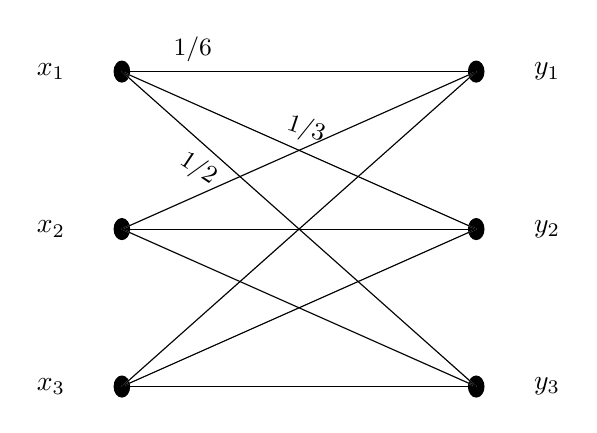
\begin{tikzpicture}[yscale=2.0, xscale=1.5] 
            % Nodi X e Y
            \foreach \i in {1,2,3} {
                \node (xl\i) at (-0.6, -\i) {$x_\i$};
                \fill (0, -\i) circle (2pt) coordinate (x\i);
                \fill (3, -\i) circle (2pt) coordinate (y\i);
                \node (yl\i) at (3.6, -\i) {$y_\i$};
            }

            % Rami di sfondo
            \foreach \i in {1,2,3} {
                \foreach \j in {1,2,3} {
                    \draw[thin, gray!30] (x\i) -- (y\j);
                }
            }

            % Rami x1 con etichette ancorate
            \draw[thin] (x1) -- node[above, pos=0.2] {\small 1/6} (y1);
            \draw[thin] (x1) -- node[above, pos=0.5, sloped] {\small 1/3} (y2);
            \draw[thin] (x1) -- node[below, pos=0.25, sloped] {\small 1/2} (y3);
            
            % Rami restanti neri
            \draw[thin] (x2) -- (y1); \draw[thin] (x2) -- (y2); \draw[thin] (x2) -- (y3);
            \draw[thin] (x3) -- (y1); \draw[thin] (x3) -- (y2); \draw[thin] (x3) -- (y3);
        \end{tikzpicture}
    \end{minipage}
    \hfill
    % --- Minipage Destra: Matrice ---
    \begin{minipage}[c]{0.40\textwidth}
        \centering
        % Dimensione standard per non farla sembrare piccola
        \normalsize 
        % Aumenta lo spazio tra le righe della matrice per matchare l'altezza del grafo
        \renewcommand{\arraystretch}{1.5} 
        \setlength{\arraycolsep}{6pt} 
        $\begin{pmatrix} 
            1/6 & 1/3 & 1/2 \\ 
            1/2 & 1/6 & 1/3 \\ 
            1/3 & 1/2 & 1/6 
        \end{pmatrix}$
        
        \par\vspace{0.3cm} % Spazio ridotto e armonizzato
        \small \textit{matrice di transizione}
    \end{minipage}
\end{center}